Inizialmente, il dataset delle traiettorie è composto da un insieme di punti aventi le seguenti caratteristiche:
una dimensione temporale espressa in secondi, due coordinate spaziali per determinare la sua posizione rispetto a un sistema di coordinate polari e
infine un identificatore di traiettoria. A queste dimensioni possono essere poi aggiunte altre informazioni, che non sono prese in considerazione durante l'esecuzione dell'algoritmo.

Scopo di questa prima fase di \textit{Cu.Te} è determinare un sistema di riferimento per i punti all'interno del dataset ed esprimere questi ultimi in
relazione al nuovo sistema.

Come indicato nella~\cref{subsec:cute:parameters}, è possibile determinare un sistema di riferimento che più aderisce alle esigenze del problema.
In questo caso la necessità principale in vista della fase di \textit{Colossal Trajectory Mining} è la ridotta dimensionalità dello spazio-tempo rispetto al numero di traiettorie
processate: si rende infatti necessario avere un numero di riferimenti spazio-temporali strettamente inferiorie alle traiettorie presenti nel database.

L'idea per risolvere questa esigenza è la divisione della superficie spazio-temporale in celle omogenee per range. Dato l'intero volume dello spazio-tempo
coperto dalle traiettorie nel dataset, questo viene partizionato in parallelepipedi di medesime dimensioni. Una cella \textit{c} è un parallepipedo, generato dal
partizionamento dello spazio-tempo coperto dalle traiettorie, avente un indice univoco.
Questa suddivisione costituisce quindi il nuovo sistema di riferimento del problema, è necessario quindi esprimere i punti all'interno del dataset rispetto a questo nuovo sistema.

Partendo dallo spazio, ogni punto di traiettoria, per definizione, determina la propria posizione sulla superficie terrestre utilizzando due coordinate, latitudine e longitudine.
Prendendo in considerazione l'area di un insieme di traiettorie, il processo per la generazione di celle spaziali è il seguente: per prima cosa si determina, mediante
il parametro \textit{s} la dimensione dei lati spaziali di una cella; successivamente si definisce la funzione \textit{pointToCell}, tale funzione ha il compito
di restituire, dato un punto, la cella di appartenenza. La cella in questione viene calcolata supponendo di scomporre la superficie terrestre in quadrati aventi lato \textit{s}
a partire da Null Island (punto avente latitudine e longituidne pari a zero)~\footnote{\url{https://blogs.loc.gov/maps/2016/04/the-geographical-oddity-of-null-island/}}.
In~\cref{fig:chap-3:milan-cell-division} è possibile vedere un esempio di divisione in celle applicato sulla città di Milano.

\begin{figure}
  \centering
  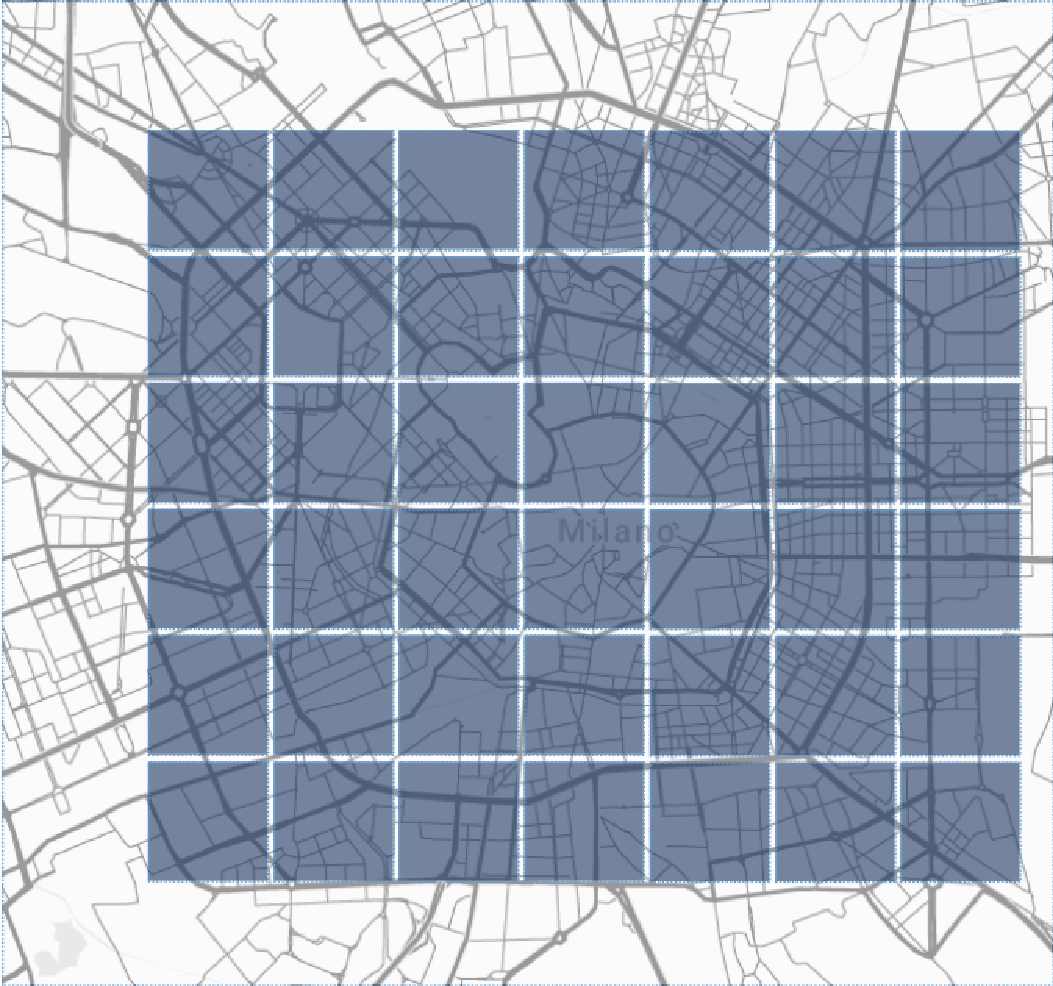
\includegraphics[scale=.6]{/sec-3/MilanCells.pdf}
  \caption{Suddivisione della città di Milano in celle,Fonte:~\url{https://which.souce?}}%
  \label{fig:chap-3:milan-cell-division}
\end{figure}

Per quanto riguarda la dimensione temporale invece, le possibilità a disposizione sono diverse, ma tra tutte si è scelto di supportare due principali scale: una basata sulle ore del giorno mentre l'altra sui giorni della settimana.
Rispetto a una metrica di tempo monotona basata su data e ora di ogni singolo punto, come ad esempio in \textit{G.C.M.P}, una scala circolare ha due vantaggi: il primo riguarda
il supporto a pattern ciclici che verrebbbero ignorati da una metrica monotona e in secondo luogo il ridotto range di valori della scala (da 0 a 23 in caso di scala giornaliera, da 0 a 6 in quella settimanale)
previene l'esplosione nel numero di celle al crescere del dataset.

Una volta determinata il lato spaziale delle celle e la durata temporale, processando le traiettorie nel dataset mediante una variazione della funzione \textit{pointToCell} adattata alla
gestione di celle tridimensionali, viene generato l'insieme delle celle \textit{C}. Questo set contiene tutte le celle, determinate dall'apposita funzione, tali che almeno
un punto di una traiettoria appartiene a quella cella. Questo approccio alla generazione delle celle garantisce che non vengano generate celle vuote, ovvero dove non passa nessuna traiettoria,
garantendo quindi una maggiore efficenza rispetto alla suddivisione assoluta della superficie spazio-temporale coperta dal dataset.

Ottenuto l'insieme delle celle, è necessario per concludere questa prima fase esprimere ogni traiettoria nel nuovo sistema di riferimento: così facendo una traiettoria non sarà più definita come
la composizione di diversi punti isolati nel tempo, ma come un'insieme di celle. La~\cref{fig:chap-3:trajectory-cell-division} mostra un esempio di conversione in un sistema di riferimento basato su celle:

\begin{figure}
  \centering
  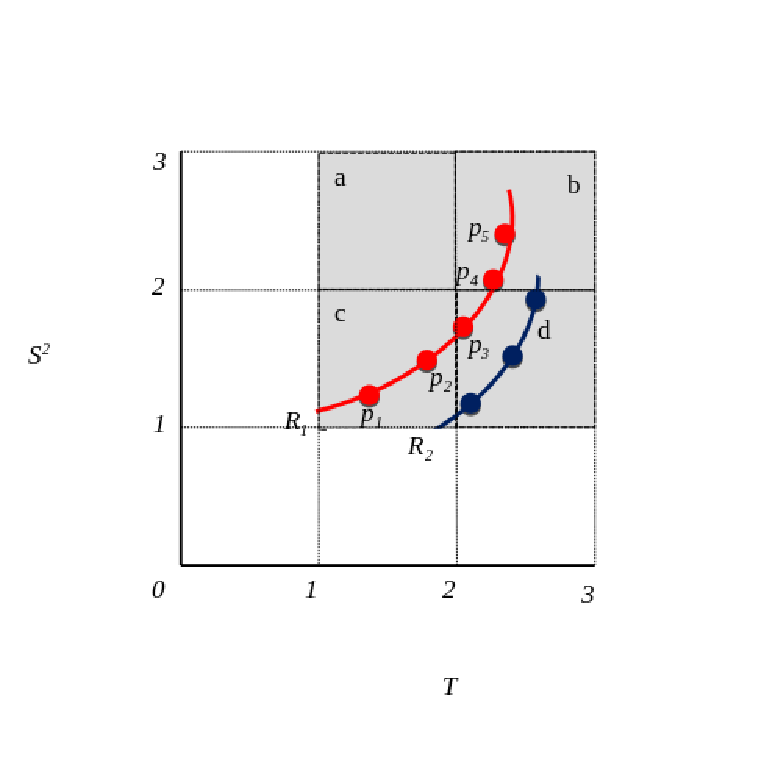
\includegraphics[scale=.8]{/sec-3/TrajectoryCellDecomposition.pdf}
  \caption{Mapping di due traiettorie, \textit{R\textsubscript{1}, R\textsubscript{2}} in un sistema di riferimento basato su celle.}%
  \label{fig:chap-3:trajectory-cell-division}
\end{figure}

Prendendo in considerazione le traiettorie \textit{R\textsubscript{1}, R\textsubscript{2}}, è possibile vedere come i punti \textit{p\textsubscript{1}, p\textsubscript{2}} appartengano alla cella \textit{c},
\textit{p\textsubscript{3}} a \textit{d} mentre \textit{p\textsubscript{4}, p\textsubscript{5}} a \textit{b}; analogamente ogni punto della traiettoria \textit{R\textsubscript{2}} sia attribuibile a \textit{d}.
Il set di celle del problema sarà quindi composto dalle seguenti celle: \textit{\textless~b, c, d \textgreater} mentre le due traiettore saranno espresse in funzione del nuovo sistema di rifermimento come segue:

\begin{itemize}

  \item \textit{R\textsubscript{1}}: \{ \textit{b,c,d} \}
  \item \textit{R\textsubscript{2}}: \{ \textit{d} \}

\end{itemize}

Va sottolineato infine che, sebbene appaia nell'immagine, la cella \textit{a} non viene effettivamente generata, poiché nessuna traiettoria ha un punto entro i suoi confini.

Una volta che le traiettorie sono state espresse nelle nuove coordinate, questo primo passo dell'algoritmo giunge a termine.

Nonostante le operazioni eseguite in questa fase possano sembrare lineari, le basi che vengono gettate influenzano l'esecuzione dell'algoritmo e gli stessi risultati finali:
tra tutte, la scelta delle dimensioni di ogni cella influenza molto i passaggi successivi. Celle piccole produrranno traiettorie lunghe, estendendo il possibile spazio di ricerca di ogni cluster.
Tanto più amplio lo spazio di ricerca, tanto più a lungo dura la sua esplorazione, tuttavia è possibile eseguire una ricerca più fine su di esso.
Lati spaziali più ampli e dimensioni temporali ridotte generano celle più grandi, con uno spazio di ricerca più ridotto e risultati più grezzi.

Nonostante quanto affermato all'inizio, non è completamente corretto dire che tutti i dati che non siano collegati alla posizione nello spazio-tempo della traiettoria siano ignorati.
È infatti possibile considerare un numero variabile di dimensioni durante il processo di generazione delle celle. Tale aggiunta infatti non fa altro che andare ad aumentare la dimensionalità della singola cella,
ciò implica un numero maggiore di celle in cui dover convertire una traiettoria, ma il risultato finale della fase sarà il medesimo, l'unica differenza sarà nell'avere mediamente traiettorie
associate a un numero maggiore di celle.

